\textbf{Ejemplo 10}\\
¿Cuánto debe crecer linealmente una serie
aritmética de 8 egresos, efectuados al final de cada período y cuyo primer egreso es de 600.000 COP para
que, puesta en valor presente, sea equivalente a una serie de 10 períodos que crecen
geométricamente en un 25\% y cuyo primer egreso es de  100.000 COP? Suponga una tasa del 2\% período
anual vencido.\\ \\
%\newpage %USAR SOLO SI EL SOLUCIÓN QUEDA SOLO Y ES NECESARIO BAJARLO A LA SIGUIENTE PAGINA
\textbf{Solución.}\\
% %La tabla ira centrada
\begin{center}
  \renewcommand{\arraystretch}{1.5}% Margenes de las celdas
%   %Creación de la cuadricula de 3 columnas
  \begin{longtable}[H]{|p{0.5\linewidth}|p{0.5\linewidth}|}
    \hline
    \multicolumn{2}{|c|}{\cellcolor[HTML]{FFB183}\textbf{1. Declaración de variables}}                 \\ \hline

    $\textit{Gradiente Aritmético}$             & $\text{Gradiente Geométrico}$                        \\
    $R =  600.000 $ COP                         & $R =  100.000 $ COP                                  \\
    $n=6 \hspace{1mm} pav$                      & $n=$                                                 \\
    $i=2\% \hspace{1mm} pav$                    & $i=2\% \hspace{1mm} pav$                             \\
    $L = ? $ COP                                & $= 25\% $                                            \\ \hline
    \multicolumn{2}{|c|}{\cellcolor[HTML]{FFB183}\textbf{2. Diagrama de flujo de caja}}                \\ \hline
    \multicolumn{2}{|p{\columnwidth}|}{ 
      % \textbf{Tabla 1}\\
      Gradiente Aritmético
      \begin{center}
          \begin{tabular}{|l|l|}
            \hline
            1  & \$ 600.000 \\ \hline
            2  & \$ 600.000 \\ \hline
            3  & \$ 600.000 \\ \hline
            4  & \$ 600.000 \\ \hline
            5  & \$ 600.000 \\ \hline
            6  & \$ 600.000 \\ \hline
            7  & \$ 600.000 \\ \hline
            8  & \$ 600.000 \\ \hline
            9  & \$ 600.000 \\ \hline
            10 & \$ 600.000 \\ \hline
          \end{tabular}
      \end{center}  
      Gradiente Geométrico
        \begin{center}
            \begin{tabular}{|l|l|}
              \hline
              1  & \$ 100.000 \\ \hline
              2  & \$ 125.000 \\ \hline
              3  & \$ 156.000 \\ \hline
              4  & \$ 195.313 \\ \hline
              5  & \$ 244.141 \\ \hline
              6  & \$ 305.176 \\ \hline
              7  & \$ 381.470 \\ \hline
              8  & \$ 476.387 \\ \hline
              9  & \$ 596.046 \\ \hline
              10 & \$ 745.058 \\ \hline
            \end{tabular}
        \end{center}   
     } \\
     
    %  \multicolumn{1}{|p{\columnwidth}|}{
    %   Gradiente Geométrico
    %     \begin{center}
    %         \begin{tabular}{|l|l|}
    %           \hline
    %           1  & \$ 100.000 \\ \hline
    %           2  & \$ 125.000 \\ \hline
    %           3  & \$ 156.000 \\ \hline
    %           4  & \$ 195.313 \\ \hline
    %           5  & \$ 244.141 \\ \hline
    %           6  & \$ 305.176 \\ \hline
    %           7  & \$ 381.470 \\ \hline
    %           8  & \$ 476.387 \\ \hline
    %           9  & \$ 596.046 \\ \hline
    %           10 & \$ 745.058 \\ \hline
    %         \end{tabular}
    %     \end{center}
    %   } \\
    \multicolumn{2}{|c|}{\cellcolor[HTML]{FFB183}\textbf{4. Aplicación de funciones}}                  \\ \hline
    \multicolumn{2}{|p{\columnwidth}|}{Para el gradiente Aritmético se aplicará la función valor presente VNA de la siguiente forma: \newline
    =VNA(0,02;B5::B12) con referencia en la hoja de Excel usada.}                                      \\
    % \multicolumn{2}{|c|}{ \includegraphics[trim=-5 -5 -5 -5 ,width=0.8\columnwidth]{10/Ejem10.png}}    \\
    \multicolumn{2}{|p{\columnwidth}|}{Para el gradiente Geométrico se aplicará la función valor presente VNA de la siguiente forma: \newline
    =VNA(0,02;E5::E14) con referencia en la hoja de Excel usada para
    el ejercicio encontrando que VP = 2.886.995 COP.}                                                  \\
    % \multicolumn{2}{|c|}{ \includegraphics[trim=-5 -5 -5 -5 ,width=0.8\columnwidth]{10/Ejem10.2.png}}  \\
    \multicolumn{2}{|p{\columnwidth}|}{Luego usando la función ‘’Buscar objetivo”, poniendo a variar L hacemos que el VP de ambos
    gradientes sea el mismo.}                                                                          \\
    % \multicolumn{2}{|c|}{ \includegraphics[trim=-5 -5 -5 -5 ,width=0.5\columnwidth]{10/Ejem10.3.png}}  \\ \hline
    \multicolumn{2}{|c|}{\cellcolor[HTML]{FFB183}\textbf{4. Respuesta}}                                \\ \hline
    \multicolumn{2}{|p{\columnwidth}|}{
    El gradiente aritmético
    debe crecer L = -60.627 COP lo que significa que el gradiente es decreciente.
    Gradiente Aritmético } \\   
    \multicolumn{2}{|p{\columnwidth}|}{
      \begin{center}
        \begin{tabular}{|c|c|}
          \hline
               Periodo (pav) & Flujo      \\ \hline
                1             & \$ 600.000 \\ \hline
                2             & \$ 539.372 \\ \hline
                3             & \$ 478.744 \\ \hline
                4             & \$ 418.117 \\ \hline
                5             & \$ 357.489 \\ \hline
                6             & \$ 296.861 \\ \hline
                7             & \$ 236.233 \\ \hline
                8             & \$ 175.605 \\ \hline
        \end{tabular}
      \end{center}
    } \\
    \multicolumn{2}{|c|}{\cellcolor[HTML]{FFB183}\textbf{5. Gráfico}}                                  \\ \hline
    \multicolumn{2}{|c|}{ 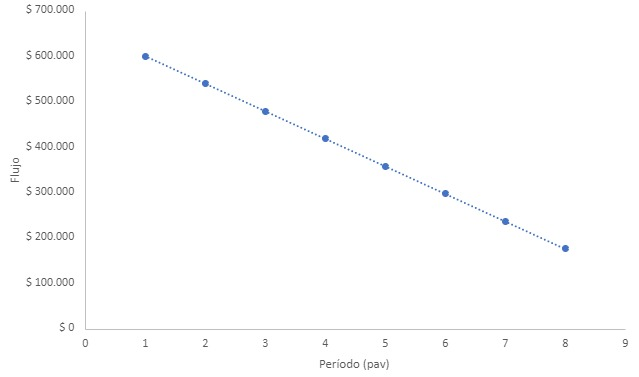
\includegraphics[trim=-5 -5 -5 -5 ,width=0.5\columnwidth]{10/grafica10.png}} \\ \hline
  \end{longtable}
%   %\newline \newline %USARLO SI CREES QUE ES NECESARIO
\end{center}